Secure Sockets Layer (SSL) and Transport Layer Security (TLS) are security
protocols for establishing a secure connection between a client and a server,
typically a web server.  This is useful to hide a clients private information,
such as credit card information or a social security number, from the public.
SSL is the predecessor of TLS and was developed by Netscape Communications
Corporation in 1994.  Later the Internet Engineering Task Force (IETF)
modified SSL 3.0 to form TLS 1.0, in 1999.  A secure connection between the
client and server is accomplished by both asymmetric and symmetric key
cryptography through a process of key exchanges, client/server authentication,
and algorithm/cipher agreements.

The process of establishing a secure connection between client and server is
done through two main components, the record protocol and the handshake protocol.  The process begins with the handshake protocol, the client creates a``Client Hello'' message that is sent to the server with a list of client supported ciphers and algorithms for hashing and comprssion.  As well as a randomly generated number, label it $r_{C}$, that will be used later in generating the symmetric key.  After the server receives the Client Hello message, it begins
comprising the ``Server Hello'' message.  This message includes a selected cipher to be used on the next message, another randomly generated number, labled $r_{S}$ and a
certification.  The certification is a way of authenticating the server to the
client or vice versa and is normally issued by a certification authority (CA).
A CA is a mutually trusted third party that verifies the identity of the
requestor; once confirmed, the CA comprises the requestor's information along
with a public key in a message to be sent \cite[p. 105]{oppliger}.  Once the Server
Hello message is received by the client, it confirms the CA that issued the
certification is on its list of trusted CAs.  Once verified, the client then
extracts the server's public key that was attached to the certification and comprises the
``Client Key Exchange'' message by creating a third random number know as the pre-master secret, label it $S_{pm}$  and encrypts
the number using the server's public key (normally using RSA) and sends the
message to the server.  Now both the server and client have the two inital random numbers($r_{C}$ and $r_{S}$) and the pre-master secret($s_{pm}$).  With this information, both the client and server can calculate master secret or symmetric key, by concatination of 

\[ MD5(s_{pm}||\text{SHA-1}(A||s_{pm}||r_{C}||r_{S})) \]
\[ MD5(s_{pm}||\text{SHA-1}(BB||s_{pm}||r_{C}||r_{S})) \]
\[ MD5(s_{pm}||\text{SHA-1}(CCC||s_{pm}||r_{C}||r_{S})) \] 

Where A, BB, CCC added for padding\cite[p. 282]{trappe}.  Before security is
concluded, one last step is taken.  Each side sends a MAC or HMAC (message
authentication code or hash message authentication code) using the random
numbers sent and the symmetric key.  MAC and HMAC are hash functions that
cannot be reversed engineered, since the functions are non-injective.  As well
as sending the MAC or HMAC, the client sends another cipher to be used on the
future messages.  This final step ensures that the information throughout the
process is constant and that there has not been an attack on the information
passed.  Once each sides checks and verifies the MAC or HMAC received, secure
communication is concluded and the two can begin sending information
securely using the record protocol\cite[p. 58]{rescorla}.

\begin{center}
    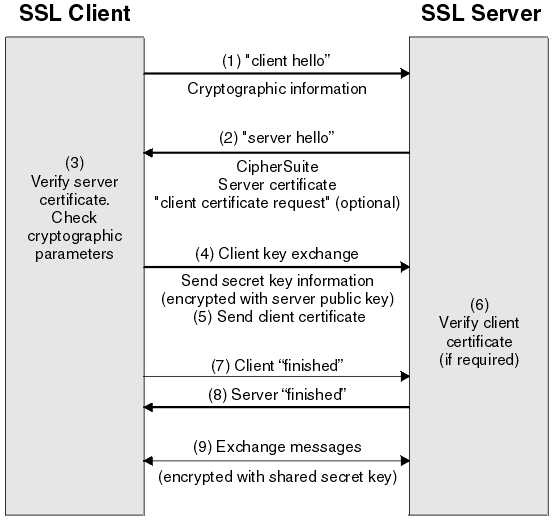
\includegraphics[width=0.75\textwidth]{SSL_TLS_Diagram.png}
\end{center}

Since SSL/TLS was developed, many attacks have succeeded in breaking its
security.  Meyer and Schwenk point out in their paper, that the protocol for
SSL/TLS should be followed and documented rigorously during implementation, and
that most of the weakness are a result of poor implementation\cite[p.
14]{meyer}.  A majority of the weakness with SSL/TLS follow from a man in the
middle attack on the Client Hello and Server Hello messages.  Because the
protocol allows for the server to pick out of a list of available client
supported ciphers, an attacker could edit this list and remove the ciphers with
higher security.  This would force the server to pick a weaker cipher or to not
allow communication.  Recent attacks have involved this process and the RC4
stream cipher in particular.  Overall, with proper implementation of the
protocol, and a strong list of ciphers,  one can assume secure communication
with SSL/TLS.
